% http://www.texample.net/tikz/examples/coin-flipping/
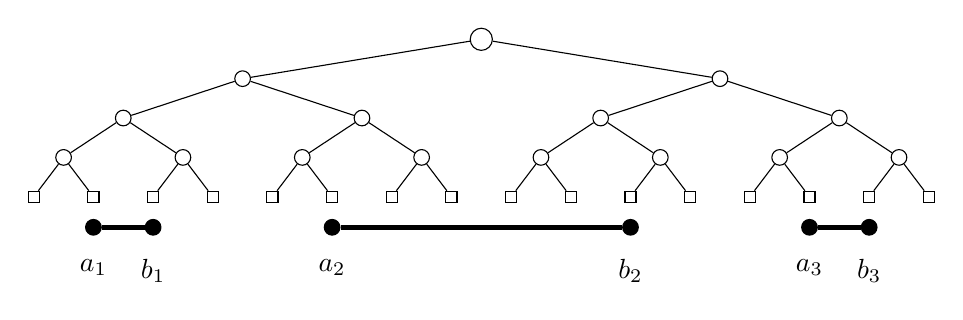
\begin{tikzpicture}[
    %scale = 1,
    %transform shape,
    %thick,
    %grow = down,  % alignment of characters
    level 1/.style = {sibling distance=\textwidth / 2},
    level 2/.style = {sibling distance=\textwidth / 4}, 
    level 3/.style = {sibling distance=\textwidth / 8}, 
    level 4/.style = {sibling distance=\textwidth / 16},
    level distance = 0.5cm,
    inner/.style = {draw, circle, inner sep=2pt},
    leaf/.style = {inner, rectangle},
    root/.style = {inner, minimum size=8pt},
    point/.style = {draw, circle, inner sep=2pt},
    truepoint/.style = {point, fill = black},
    falsepoint/.style = {point, fill = white},
    trueinterval/.style = {line width = 2pt}
  ]
  \node[root] (eps) {}
   child {   node[inner] (0) {}
     child { node[inner] (00) {}
       child { node[inner] (000) {}
         child { node[leaf] (0000) {}}
         child { node[leaf] (0001) {}}
       }
       child { node[inner] (001) {}
         child { node[leaf] (0010) {}}
         child { node[leaf] (0011) {}}
       }
     }
     child { node[inner] (01) {}
       child { node[inner] (010) {}
         child { node[leaf] (0100) {}}
         child { node[leaf] (0101) {}}
       }
       child { node[inner] (011) {}
         child { node[leaf] (0110) {}}
         child { node[leaf] (0111) {}}
       }
     }
   }
   child {   node[inner] (1) {}
     child { node[inner] (10) {}
       child { node[inner] (100) {}
         child { node[leaf] (1000) {}}
         child { node[leaf] (1001) {}}
       }
       child { node[inner] (101) {}
         child { node[leaf] (1010) {}}
         child { node[leaf] (1011) {}}
       }
     }
     child { node[inner] (11) {}
       child { node[inner] (110) {}
         child { node[leaf] (1100) {}}
         child { node[leaf] (1101) {}}
       }
       child { node[inner] (111) {}
         child { node[leaf] (1110) {}}
         child { node[leaf] (1111) {}}
       }
     }
   };

  % Labels
  \begin{scope}[nodes = {draw = none}]
    \begin{scope}[nodes = {below = 8pt}]
      \node [name = a1, truepoint] at (0001) {};
      \node [name = b1, truepoint] at (0010) {};
      \draw [trueinterval] (a1) -- (b1) node {};
      \node [name = a2, truepoint] at (0101) {};
      \node [name = b2, truepoint] at (1010) {};
      \draw [trueinterval] (a2) -- (b2) node {};
      \node [name = a3, truepoint] at (1101) {};
      \node [name = b3, truepoint] at (1110) {};
      \draw [trueinterval] (a3) -- (b3) node {};
    \end{scope}
    \begin{scope}[nodes= {below = 8pt}]
      \node at (a1) {$a_1$};
      \node at (b1) {$b_1$};
      \node at (a2) {$a_2$};
      \node at (b2) {$b_2$};
      \node at (a3) {$a_3$};
      \node at (b3) {$b_3$};
    \end{scope}
  \end{scope}
\end{tikzpicture}